% Introduction au projet quantrade à l'intention des chefs sioux
% version 0.1
% 2013-03-22
% par Xavier Bruhiere (xavier.bruhiere@gmail.com)
% Ce document est mis  disposition selon le Contrat "Creative Commons Paternité-Partage des Conditions Initiales  l'Identique 3.0 Unported"
% http://creativecommons.org/licenses/by/3.0/


\documentclass[12pt,a4paper]{article}
%Chargement des packages
\usepackage[utf8]{inputenc} % l'encodage des fichiers est utf-8, mettre [latin1] si necessaire
\usepackage[french]{babel} %le rapport est en français 
\usepackage{amsmath}
\usepackage{amsfonts}
\usepackage{amssymb}
\usepackage{graphicx} %pour afficher des images
\usepackage{float}	%pour forcer le placement des images.
\usepackage{geometry} %pour la modification des marges
\usepackage{fancyhdr} %pour modification des pieds de page
\usepackage{longtable}
\usepackage{listings}
\usepackage{subfigure}
\usepackage{hyperref} %pour que les références soient des liens hypertextes
\usepackage[usenames,dvipsnames]{color} % pour les textes en gris


\newcommand{\TitreRapport}{Projet QuanTrade - Quantitative and collective trading intelligence}
\newcommand{\DateRapport}{2013}
\newcommand{\AuteurRapport}{Xavier Bruhiere}
\newcommand{\NomEntreprise}{QuanTrade}

% Subsubsubsection fixing
\setcounter{secnumdepth}{5}

%définition des marges
\geometry{hmargin=2.5cm, vmargin=2.5cm } 

%utilisation des puces anglaises.
%attention, il faut avoir une version récente de frenchb.ldf. 
\frenchbsetup{StandardItemLabels}

%Définition des en-têtes et pieds de page
\renewcommand{\headrulewidth}{0pt}
\renewcommand{\footrulewidth}{0pt}
\fancyhead[C]{ \textcolor{Gray}{\small\TitreRapport}}
\fancyfoot[C]{ \textcolor{Gray}{ \small\AuteurRapport ~~ \vline ~~ QuanTrade ~~ \vline ~~ \DateRapport }}

\fancyfoot[LE, RO]{\thepage}
\fancyfoot[RE,
LO]{
\includegraphics[width=1.8cm]{style/images/wall-street.jpg}}

\fancyhead[L,R]{}


% définition du tire, de la date et de l'auteur du document
\title{\TitreRapport}
\date{\DateRapport}
\author{\AuteurRapport}

\makeatletter

\renewcommand\maketitle{
  \begin{titlepage}
  	\begin{center}
    	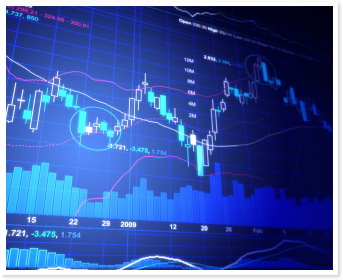
\includegraphics[height=3cm]{images/graph.png}
    	\hspace{\stretch{1}}
    	
\includegraphics[height=3cm]{images/forex-trading.jpg}
    
    \vspace{\stretch{0.5}}
    	
		  \begin{tabular*}{1.0\textwidth}{l @{\extracolsep{\fill}} r}
					Start Up 				& \NomEntreprise 				\\
					Projet d'entreprenariat \@date 							&
          Paris/Londres/Worldwide 		\\
			\end{tabular*}

  	\vspace{\stretch{1.5}}
  	
 		{\large \bf Introduction au projet \\}
    \vspace{0.5cm}
    {\LARGE \bf \@title\\}
    \vspace{0.5cm}
    {\large \it \@author\\}
  
	  \vspace{\stretch{2}}
	  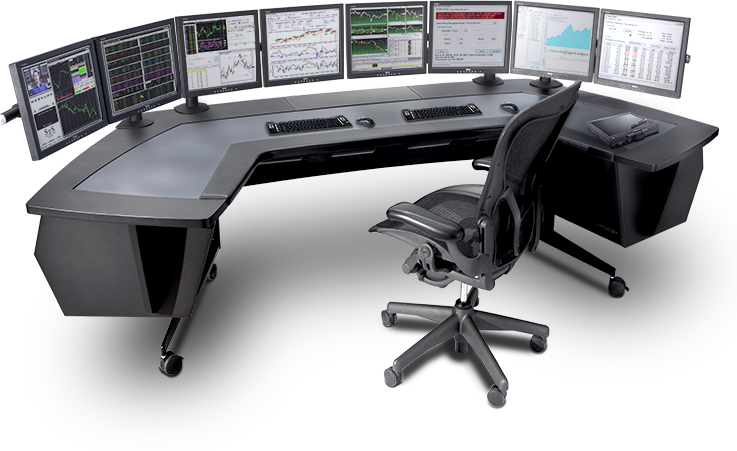
\includegraphics[width=1.0\textwidth]{images/TradingDesk.png}
	  \vspace{\stretch{2}}

    \newpage


	  \vspace{\stretch{2}}
	  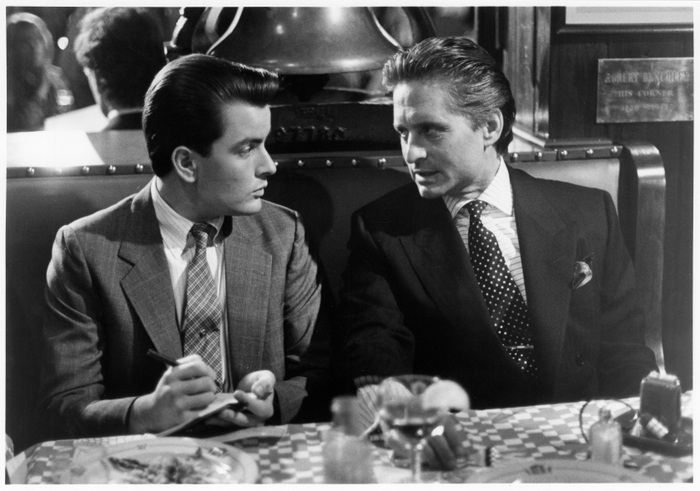
\includegraphics[width=1.0\textwidth]{images/wallstreet.jpg}
	  \vspace{\stretch{2}}

    \newpage

  \end{center}\par
  \end{titlepage}
  \setcounter{footnote}{0}
  
%  \global\let\thanks\relax
%  \global\let\maketitle\relax
%  \global\let\@thanks\@empty
%  \global\let\@author\@empty
%  \global\let\@date\@empty
%  \global\let\@title\@empty
%  \global\let\title\relax
%  \global\let\author\relax
%  \global\let\date\relax
%  \global\let\and\relax
}


\makeatother


\begin{document}
\pagestyle{fancy}

\maketitle
		\newpage
\section*{Résumé :}


		\newpage
\tableofcontents
        \newpage
\section{Opportunités}

\subsection{Open-source/data}

\begin{minipage}[c]{10cm}
  L'informatique explose et tous les moyens sont bons pour développer de plus
en plus efficacement et à moindre coup, comme pour l'électronique. Dans la
foulée du mouvement les équipes de passionnés se forment et développent
aussi efficacement que les grands groupes. Le modèle économique est
discutable, mais l'association de milliers de compétences transnationales
cartonnent sans aucun doute.\newline
Reste à posséder des outils puissants : check ! Git, OpenERP (clin d'oeil
Mahtieu), linux embarqué, vim (clin d'oeil à moi) \ldots \newline
\newline
Pour être plus concret voici quelques exemples que j'avais mailé il n'y a
pas longtemps qui illustrent ce que peut produire d'élitiste les
communautés de passionnés et les sciences libres. \newline
\end{minipage}

\begin{itemize}

    \item Quantopian
  Il s'agit d'une toute nouvelle société qui propose à l'heure actuelle de
réaliser sur leur site web des simulations quantitatives de trading. Elle
est remarquable sur 2 points: Leur moteur de backtest open-source que
j'utilise entièrement,  en sa qualité de béta-testeuse du marché. En effet je partagent leur vision
et leur méthode de travail et en ce sens il est très intéressant de voir
comment est reçu leur offre. \newline
On parle d'un public très élitiste (programmeur en finance quantitative),
mais on peux déjà voir qu'ils ont 4 business angels, 80 contributeurs actifs et 700
suiveurs pour la partie code, et certains posts ont été lus par plus de 1000
membres. En outre la photo suivante qui cartographie les contributeurs sur
leur site sur 24H parle d'elle-même.\newline
\newline
%%%%%%%%%%%%%%% Include graphique %%%%%%%%%%%%%%%%

  \item Coursera, Udacity, Edx
    Les cours en ligne des grandes universités sur lesquels je me suis
formé en programmation, finance, gestion de portefeuille, analyse de
donnée, modélisation de marché, traitement naturel du langage et
extraction de l'information web. Je n'ai malheureusement pas les
chiffres par cours, mais je sais que celui sur l'intelligence
artificielle, un des premiers, a été suivi par plus de 250 000
personnes. Toujours sur la base de la motivation et de l'initiative
personnelle: les gens sur ces forums sont chauds patate !\newline

  \item R-bloggers
    R c'est le langage le plus puissant pour tous ce qui est relié au
calcul statistique, et r-bloggers c'est LE site ou des contributeurs (450
professionnels à cette heure) viennent publier leurs recherches. 8 articles
hier dont 3 concernant la finance (2 en gestion de portefeuille et interface
web, un sur les réseaux de neurones). Si je fais une recherche avec 'trading'
j'obtiens 379 tutos et articles de niveau R&D (j'en ai trouvé écrits récemment par
l'actuel directeur de la recherche chez google !). Et j'ai écrit l'interface
qui permet de les intégrer au projet.\newline
\newline
\end{itemize}


L'intérêt ici est de se rendre compte qu'en capitalisant toutes ces
ressources intelligentes il devient possible d'aller plus encore en avant dans
l'utilisation des technologies pour résoudre des problèmes plus complexes
(au hasard : prédire les cours de la bourse de demain).\newline
\newline

A l'heure du 21iem siècle ces problèmes impliquent des volumes de data
colossaux., non triviaux à gérer et traiter.


  \item Bloomberg
    le leader de l’information sur les marchés, a rendu
gratuit l'accès à ses données.  Quandl est un nouveau moteur de recherche qui
vise à centraliser et à rendre accessible les bases de donnée du web.  Depuis
google finance, ou avec TrueFX, les quotes des marchés sont accessibles temps
réel ! (bien que j'y sois allé un peu fort une fois et qu'il m'ait banni
pendant 1h ^^).  Sans parler des prédicteurs, estimateurs, ... que je vous ai
montrés hier.  Tous les grands services web (facebook, twitter, ...) ont créé
des APIs qui permettent de récupérer gratuitement leurs données.  La NASA, le
CNRS, l'INRIA, ... rendent leur thèses et datacenter accessibles !  J'vais
pas tout cité mais on rentre dans l'ère de l'open data et de l'OSINT, et ça
c'est de l'or pour qui sait les traiter !

\subsection{Technologies}

\subsection{La finance quantitative}

% section Opportunites (end)

\newpage

\section{Business Model}


\subsection{A contre-pied}
\label{sub:A contre-pied}

\subsection{La data}
\label{sub:La data}

\subsection{Bank bonus}
\label{sub:Bank bonus}


% section Business Model (end)

\newpage

\section{Roadmap}


\subsection{Live-trading}
\label{sub:Live-trading}

\subsection{Communication et et préparation}
\label{sub:Communication et et préparation}

\subsection{Investisseurs et start-up}
\label{sub:Investisseurs et start-up}


% section Roadmap (end)


		\newpage
\section*{Conclusion}
\addcontentsline{toc}{section}{Conclusion}


La première version de QuanTrade est déjà bidouillée par des contributeurs,
les tests seront bientôt finalisés, et la version live sera mise
en route à 9h30 à l'ouverture du marché. Autrement dit le plus pénible est terminé et il est temps
d'utiliser tout ce code pour aller chercher des pépettes et des sujets de
recherche géniaux.\newline

A présent, parallèlement à la poursuite du développement, la communication
auprès des communautés open-source et étudiantes va commencer, de même que
la formalisation du business model (qui transpire d'un peu partout de ce
document) et de fait la recherche de financement.\newline

A en juger par les articles dans Forbes ou dans le New-York Times, au
succès fulgurant de quantopian, à la qualité des ressources en
connaissances et en projets libres, il y a un énorme pari à faire, passionnant à mener.\newline

Il ne reste plus qu'à répondre à mon mail pour récupérer tes accès au tableau
de bord, et à venir boire une bière cette semaine pour passer aux
choses sérieuses !

    \newpage
\end{document}
